%!TEX root =  ../main.tex

\chapterimage{\chapdir/pics/PIA05380} 
\mychapter{Identities}{identities}

Trigonometry is like the Hydra of ancient legends: you cut off one head, only to have
three more erupt out.  The interrelated nature of the circle and the reference triangle
mean there are an infinite number of ways to express the same function, via
trigonometric functions.


\newpage
\chapterminitoc


%									10 - 1
\newpage
\invisiblesection{Simple Trigonometric Equations}
\subsection{Lab}
\noindent\makebox[\textwidth]{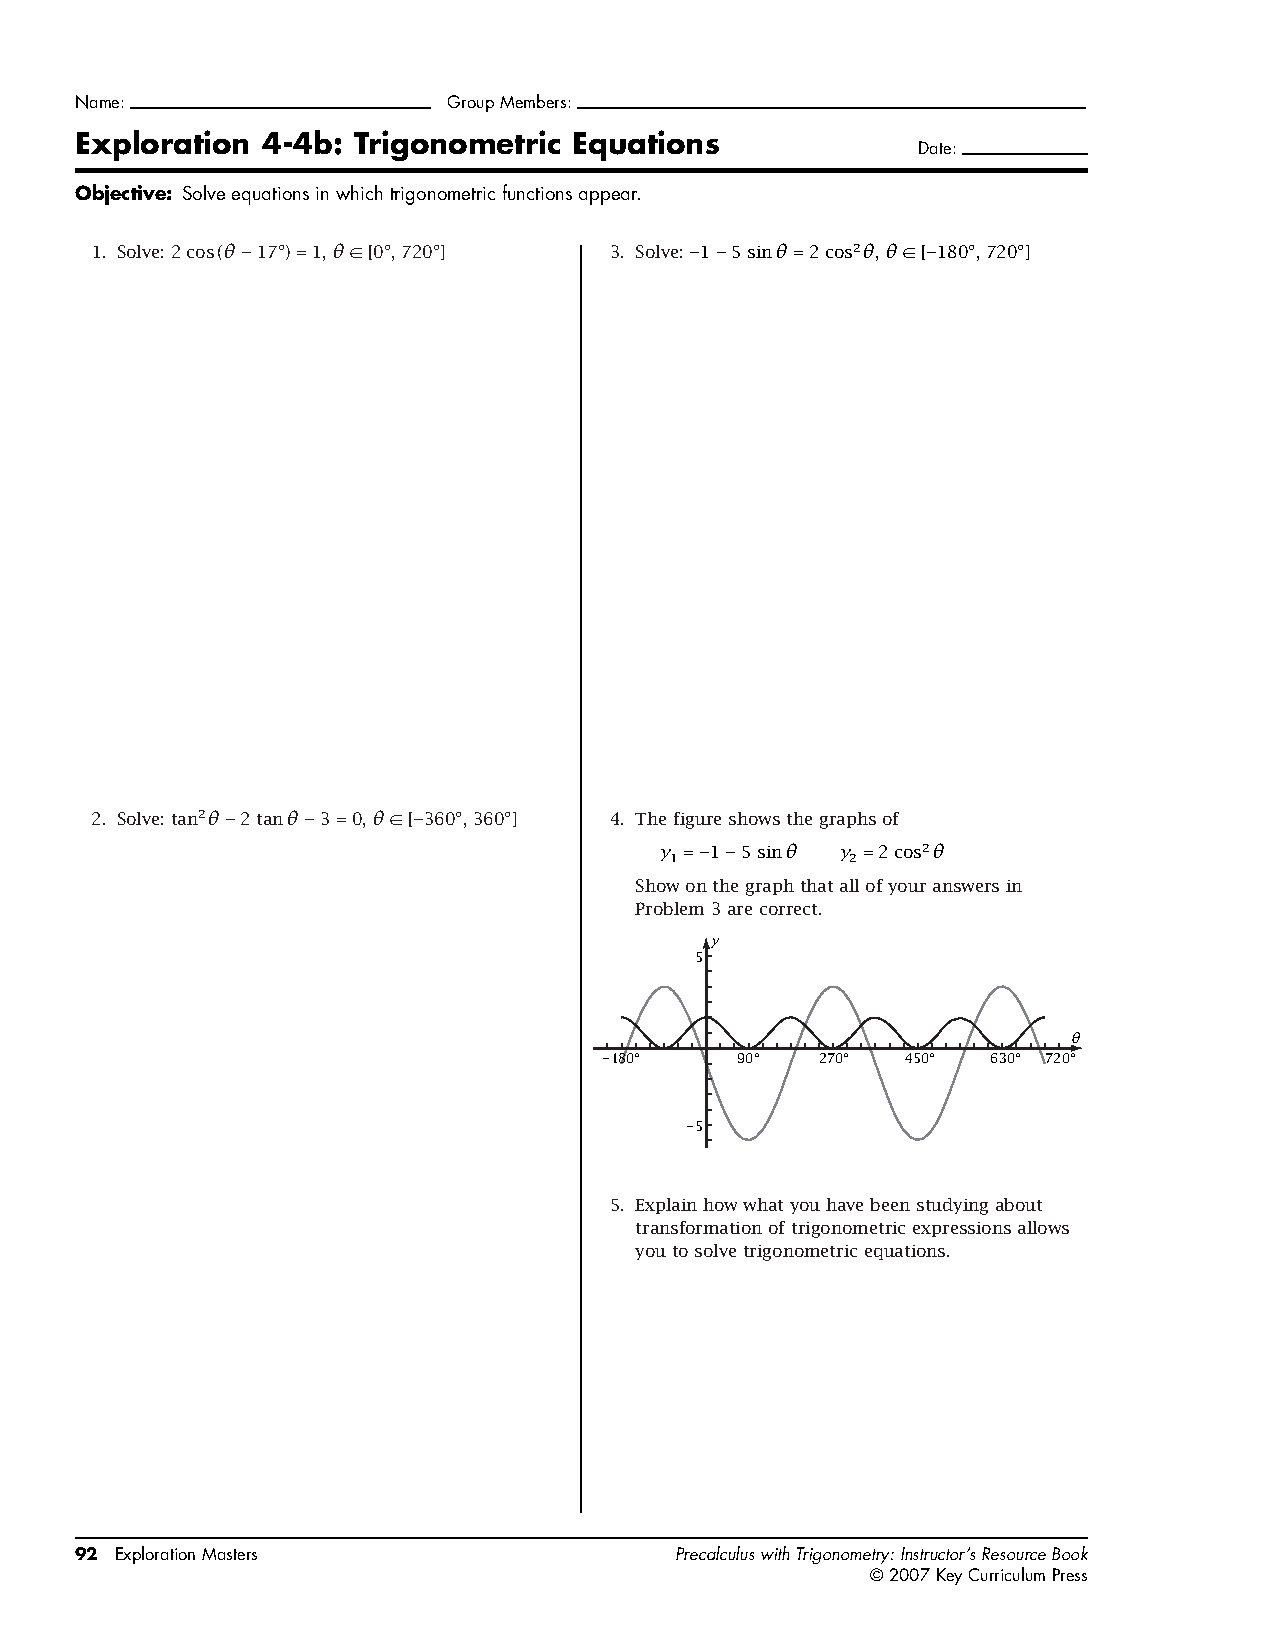
\includegraphics[width=\paperwidth]{ch10/1001p.pdf}}
\subsection{Sine Slices}
Trigonometric equations are unlike linear equations, in that they have infinitely many
answers.  We typically answer them over a domain like $\theta \in \left[0,\tau\right]$ or
$\theta \in \left[\-\frac{\tau}{2},\frac{\tau}{2}\right]$.  Let us begin by finding a way to
express the infinite solution set.

\marginfig[-0.5in]{\chapdir/pics/Sin_unit_circle.png}{The height achieved by turning 
angle $\alpha$ will reoccur in one other place\label{fig:sinecircle}.}
Suppose we want to find all the answers to a simple equation
\begin{equation}\label{eq:sinx12}
\sin(x) = \frac{1}{2}
\end{equation}
With the Unit Circle memorized, we can easily recall that this happens at 
$\frac{\tau}{12}$.  However, we know that sine is $y$ on the Unit Circle, and so it
will come up again and again.  As Fig.~\ref{fig:sinecircle} shows, the height will
reoccur at $\frac{\tau}{2}-\theta$.  We also can add or subtract as many full-rotations
(i.e. $\tau$) as we like, and still get the same height.  This means that the full
solutions set for Eq.~\ref{eq:sinx12} is
$$
x  = \begin{cases} \frac{\tau}{12} & \pm k\tau\\
\frac{11\tau}{12} & \pm k\tau \end{cases} 
$$
where $k \in \mathbb{W}$Or the more general solution for $\sin\theta=x$:
\begin{equation}
\theta  = \begin{cases} \sin^{-1}(x) & \pm k\tau\\
\frac{\tau}{2} - \sin^{-1}(x) & \pm k\tau \end{cases} 
\end{equation}
Notice that only if $\sin^{-1}(x)$ is known can these be resolved without a
calculator.

\subsection{Cosine Cuts}
\marginfig[0in]{\chapdir/pics/Cos_unit_circle.png}{The horizontal displacement 
achieved by turning  angle $\alpha$ will reoccur in one other place\label{fig:cosinecircle}.}
Substitution can help prevent confusion when there is junk like (e.g. $\theta-17$) inside
There can be quadratics etc, which substitution make clearer.
\subsection{Tangent Tilts}
The period can be off, so consider making a general solution and using it to generate answers
\newpage
\subsection{Exercises}
to be done in Kuta


%									10 - 2
\newpage
\section{Co-function, Pythagorean, Even/Odd}
\subsection{Problems}
To be done in Word.
Count sides as sin, cos, 1.  Pythagorus
Draw right triangle.  Use theta and 90-theta.  Side of x, y, r.  find sine and cosine of each
\newpage
\subsection{Reference Triangle Within}
\subsection{Reference Triangles Without}
\subsection{Full Geometry}
\subsection{Algebra Ratios}
\subsection{Time Savers}
\subsection{Conjugates}
\newpage
\subsection{Exercises}
Use the Pythagorean identities to produce/solve ellipses and hyperbolas - to be do


%									10 - 3
\newpage
\invisiblesection{Sum and Difference Identities}
\subsection{Problems}
Make rectangles in Word --- to be done
%\noindent\makebox[\textwidth]{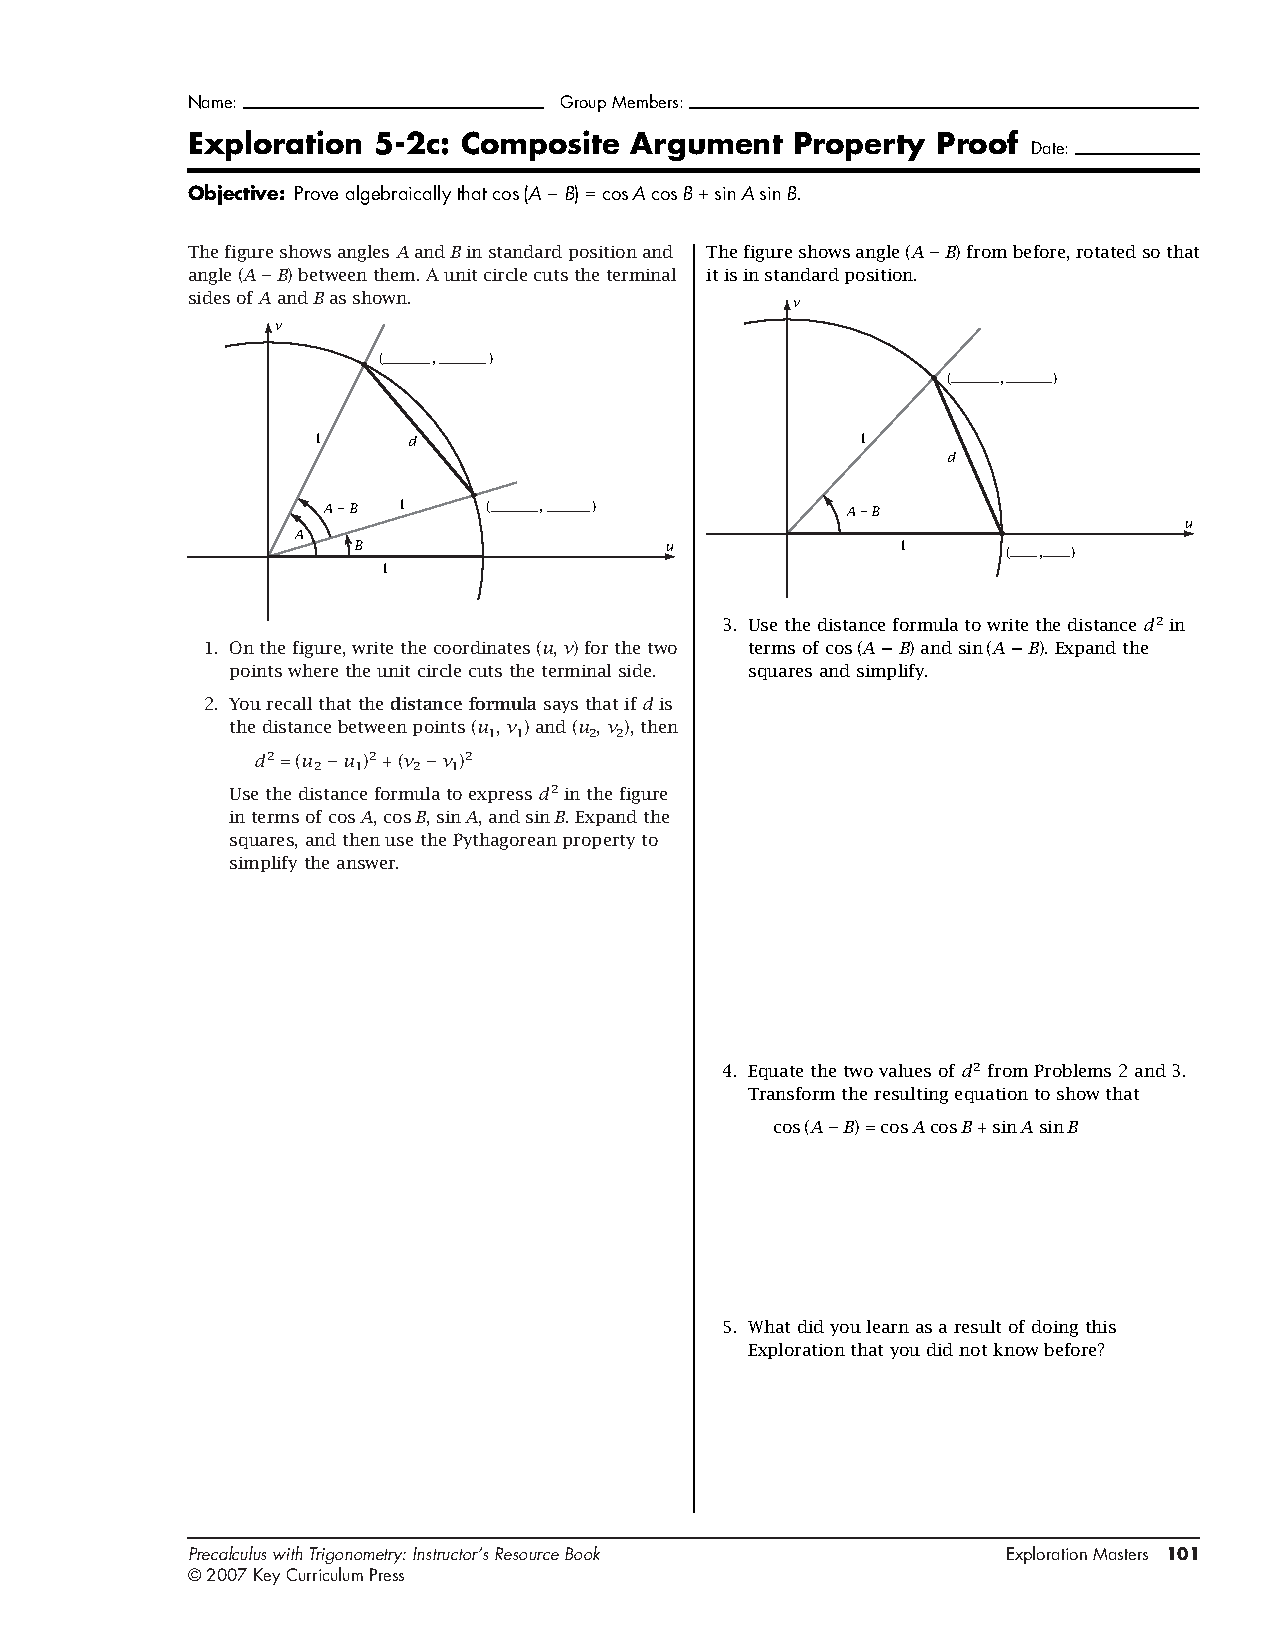
\includegraphics[width=\paperwidth]{ch10/1004p.pdf}}
\subsection{Cosine Sum and Difference}
\subsection{Sine Sum and Difference}
\subsection{Tangent Sum and Difference}
\newpage
\subsection{Exercises}
to be done in Kuta


%									10 - 4
%\newpage
\invisiblesection{Double Angles}
\subsection{Problems}
\noindent\makebox[\textwidth]{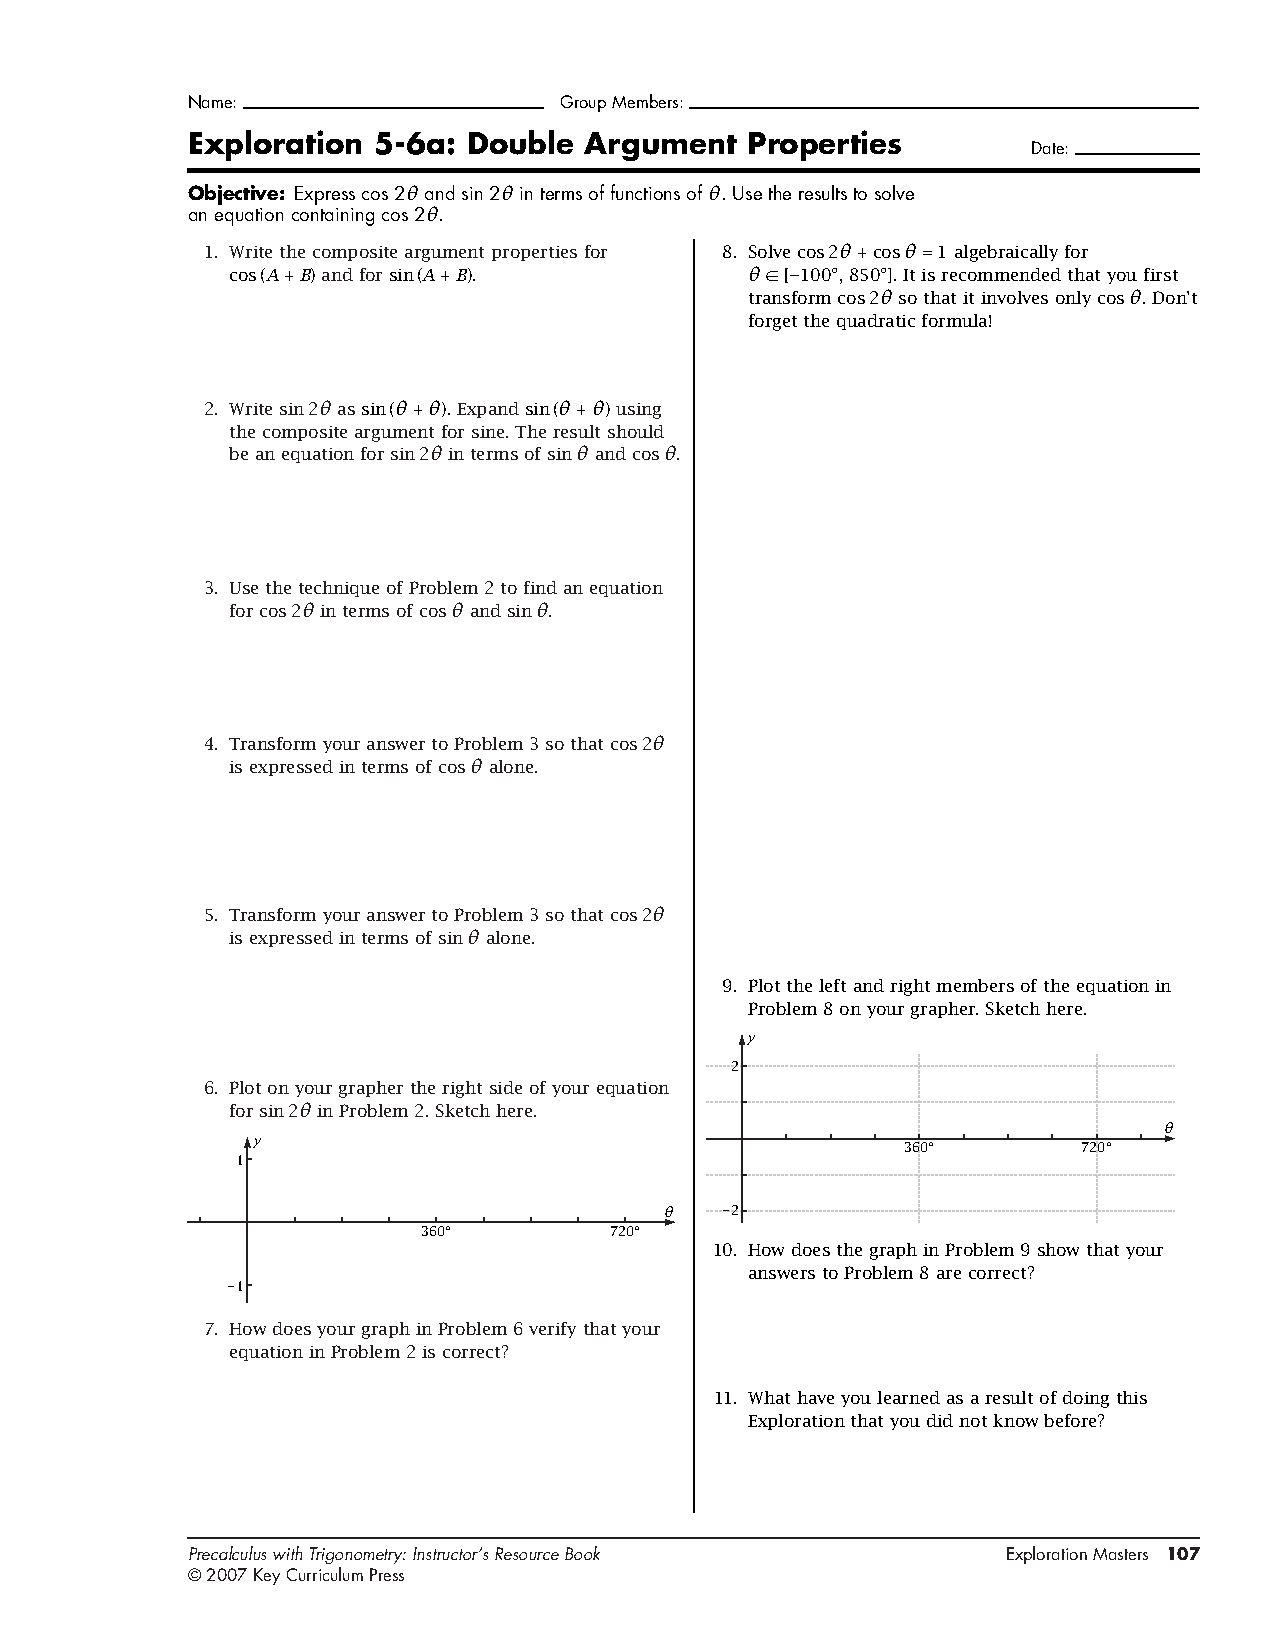
\includegraphics[width=\paperwidth]{ch10/1005p.pdf}}
\subsection{Double Sine}
\subsection{Double Tangent}
\subsection{Double Cosine}
\subsection{Half and Power}
\newpage
\subsection{Exercises}
to be done in Kuta


%									10 - 5
\newpage
\section{Proofs}
\subsection{Problems}
to be done in word
\newpage
\subsection{Summary of Trigonometric Derivatives}
\subsection{Summary of Trigonometric Integrals}
\subsection{Summary of Trigonometric Identities}
\subsection{Techniques for Proofs}
\newpage
\subsection{Exercises}
Prove that the area of a circle is pi r squared
\index{area!of a circle as an integral}
Prove that the area of an ellipse with radii a, b is abpi
\index{area!of an ellipse as an integral}
to be done in word


\newpage
\section{Review}
\subsection{Chapter Review}
\subsection{Chapter Test}